Centrality is a measure which indicates the importance of a node. The degree of a node is the most common and basic measure in the field of network analysis. The degree centrality counts the number of paths of length 1 that emanate from a node. Another degree centrality measure instead is the PageRank, which simulates a random walk on the graph. The rank gives the probability a surfer reaches the respective page. 

The second group of centrality measures is the group of diameter related measures, which count the length between nodes. The closeness for example takes the diameter into account in order to identify a nodes’ importance. A general definition of closeness is based on the length of the average shortest path between a node and all other nodes in the network. 

The third measure is the betweenness which considers the flow. A general definition of the betweenness is the number of node pairs that need to go through a node in order to reach each other taking the minimum number of hops. Figure \ref{fig1} shows the three groups of measures.

\begin{figure}[H]
	\begin{center}
		\label{fig1}		
		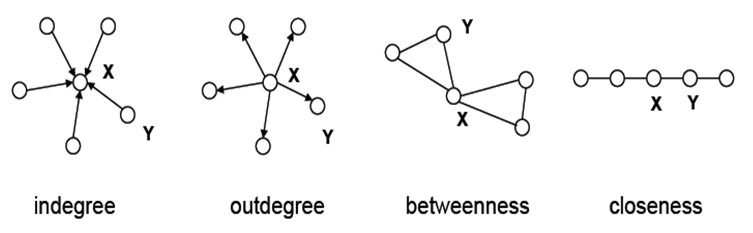
\includegraphics[width=0.6\textwidth]{fig1}	
		\caption{Measures overview}	
	\end{center}
\end{figure}

\subsection{Degree, indegree and outdegree}
The degree is a fundamental measure within the analysis of networks. It gives some indication of a nodes position in the network. The indegree of a vertex in a directed graph is given by the number of edges pointing to the respective vertex. The outdegree on the contrary gives the number of edges coming from the corresponding node. In order to efficiently compute the both degrees, we build the adjacency matrix of the network and count the neighbors of node with MapReduce.

\subsection{Degree distribution}
The degree distribution is the probability distribution of the degrees over the whole network. This project scalable computes them by using the MapReduce model using the degree as key in a key-value pair. The subsequent reduce job builds the sum of these key-value pairs and so builds the degree distribution.

\subsection{PageRank}
The PageRank algorithm was developed by Google founders Larry Page and Sergej Brin at Stanford University in 1996. The algorithm is used to rank pages in order to measure the importance of websites. Therefore, the algorithm computes a probability distribution representing the likelihood that a user reaches a specific web page by randomly clicking on links. In order to compute the PageRank, we run the algorithm in iterations. To handle circles in the graph, which might prevent the algorithm from converging, we implemented the random teleport behavior. At each node there is a certain probability that the random surfer "teleports" to another node randomly. Further, nodes without outgoing edges constitute a serious problem that has to be handled. There are several possibilities to tackle this issue. In this project nodes without outgoing edges have been modified in a way that these point to all other nodes in the network visualized as green arcs in Figure \ref{fig2}.

\begin{figure}[H]
	\begin{center}
		\label{fig2}		
		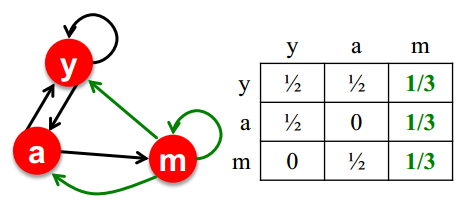
\includegraphics[width=0.75\textwidth]{fig2}	
		\caption{PageRank sinks}	
	\end{center}
\end{figure}

\subsection{Closeness centrality}
Closeness measures the importance of a node based on the distance to other nodes in the network. The intuition of the large-scale algorithm is to count approximately the number of neighbors that a node connects to at each step of the iterative computation. This approach is proposed by Kang et al. in their paper “Centralities in Large Networks: Algorithms and Observations” [1]. Effective Closeness is a large-scale centrality algorithm. 

Following Figure \ref{fig3} shows a toy example showing the intuition. For node 1, at step 1, it connects to two nodes, at step 2, it connects to two nodes and at the final step, it  connects one node. Therefore, node 1’s count is given by 1 * 2 + 2 * 2 + 3 * 1 = 9. For node 3, the count is 3 * 1 + 2 * 2 = 7. It is observable that node 3 is more central than node 1. The closeness supports this since node 3’s count is less than node 1’s count. Note that the closeness does not consider the direction of edges.

\begin{figure}[H]
	\begin{center}
		\label{fig3}		
		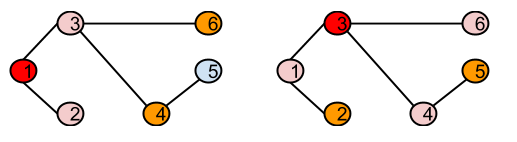
\includegraphics[width=0.6\textwidth]{fig3}	
		\caption{Closeness}	
	\end{center}
\end{figure}

The other scalable skill applied is the count distinct elements skill in data stream which is called Flajolet-Martin (FM).  When observing a stream of random integers, see an integer which binary representation starts with limited buckets, there is a higher chance that the cardinality of the stream is 2\^\ (size of the limited buckets). For instance, 25\% of bits start with "01", 12,5\% starts with "001" and if the limited bucket show "001", the estimated cardinality is 8. Thus, effective closeness algorithm uses bitstring to represent nodes and update the next step with bitwise OR. 

Originally, the algorithm is designed for undirected graphs, thus, this project firstly transforms the directed Hyperlink Graph into an undirected graph, and then applies the described algorithm on it.

\begin{figure}[H]
	\begin{center}
		\label{fig4}		
		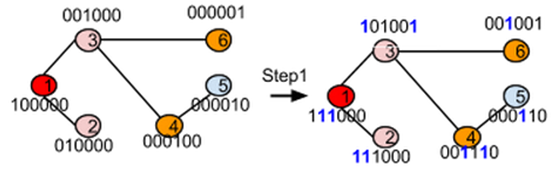
\includegraphics[width=0.6\textwidth]{fig4}	
		\caption{One step of closeness computation}	
	\end{center}
\end{figure}

\subsection{Betweenness centrality}
The betweenness centrality of a node in a network is given by the number of shortest paths from any other node to another node that passes the respective node. It is therefore an indicator of a nodes’ importance or centrality. To calculate it, the intuition is to score each edge by “power iteration” and then calculate the importance of nodes by aggregating the edges’ score. This approach is as well proposed by Kang et al. in the paper “Centralities in Large Networks: Algorithms and Observations”. For the Hyperlink Graph in this project, the implementation pre-processes the graph by removing dead-ends and transform the directed graph into undirected graph.

\begin{figure}[H]
	\begin{center}
		\label{fig5}		
		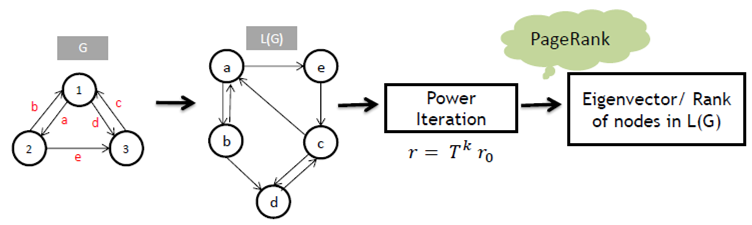
\includegraphics[width=1.0\textwidth]{fig5}	
		\caption{Betweenness}	
	\end{center}
\end{figure}

The intuition of the betweenness, which is also called LinkRank, is that some edges are important since many nodes have to go through them to reach other nodes. This flow-based measure is similar to the main road and branch approach. Nodes that connect to the main roads are more important. Thus, the scalable calculation of the betweenness uses similar measures to the PageRank way in order to identify more important edges in the network.

Based on the description above, the first step is to transform the graph G into a line graph L(G) where nodes become arcs and edges become nodes, respectively. The scalable idea here is instead of materializing L(G), decomposing L(G) by S(G) x T(G) which are in-edges and out-edges. 

\begin{figure}[H]
	\begin{center}
		\label{fig6}		
		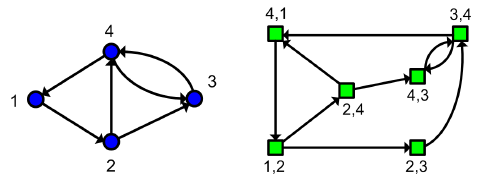
\includegraphics[width=0.8\textwidth]{fig6}	
		\caption{Graph G and its line graph L(G)}	
	\end{center}
\end{figure}

\begin{table}[t]
	\caption{S(G) and T(G)}
	\label{t1}
	\begin{center}
		\begin{tabular}{|l|l|l|l|l|l|}
			\hline
			S(G)	&	&	&T(G)	&	&	\\ \hline
				&source	&	&	&target	&	\\	\hline
			arc1	&1	&1	&arc1	&2	&1	\\ \hline
			arc2	&2	&1	&arc2	&3	&1	\\ \hline
			arc3	&2	&1	&arc3	&4	&1	\\ \hline
			arc4	&3	&1	&arc4	&4	&1	\\ \hline
			arc5	&4	&1	&arc5	&1	&1	\\ \hline
		\end{tabular}
	\end{center}
\end{table}

The next step in the computation is the calculation of the eigenvector S(G) multiplied by T(G) which is the same as the PageRank which is given by the stationary probability. After finishing the computation of the arcs importance score, the scores are summed up to retrieve the final LineRank score for each node T.